% ===================================================================
\section{Device: conditional modeling and calibration}\label{sec:device}
% ===================================================================
\begin{rulebox}\textbf{Construction and procedure NOT verified.} The 2027 Rules Manual, official clarifications, and tournament instructions were not available to this build (official site blocked from the build environment; nothing attached). Unverified search \emph{snippets} conflict: the official event description reportedly says teams build a device ``designed to \textbf{collect} heat'',\src{SO1}\src{SO2} while a community wiki describes an insulated-beaker \textbf{heat-retention} task (hot water in a beaker, timed loss).\src{WIKI} Do not build, modify, or plan testing from this page. Read the official rules for: allowed materials and energy sources, dimensions, what is measured and when, scoring variables, required prediction or documentation, and impound. This section contains only physics that holds under either reading. Construction changes require rule review and fresh validation; this binder does not recommend an overnight rebuild.\end{rulebox}

\begin{multicols}{2}
\subsection{Single-node energy balance}\label{sec:devicemodel}
\CORE{}
\begin{formulabox}
\begin{equation}
C_{\text{eff}}\,\frac{\dd T}{\dd t}=P_{\text{in}}(t)-K\,(T-T_{\text{amb}})-\dot Q_{\text{other}} \label{F:device:balance}
\end{equation}
\end{formulabox}
$C_{\text{eff}}$ = total heat capacity that moves with the measured temperature (water + inner container + probe; \si{J/K}); $K$ = overall loss conductance (\si{W/K}; $1/K$ = total network resistance, \sref{sec:resistances}); $P_{\text{in}}$ = absorbed input power (zero for pure retention); $\dot Q_{\text{other}}$ = evaporation and other losses not proportional to $T-T_{\text{amb}}$.

\textbf{Assumptions:} one well-mixed temperature; constant $C_{\text{eff}}$, $K$, and $T_{\text{amb}}$ over the run (radiation and natural convection make $K$ rise slightly with $T$); no phase change; device parts not in the node either negligible or lumped into $K$.

\textbf{Solutions:} constant $P_{\text{in}}$: \eqp{F:transfer:input}; no input: \eqp{F:transfer:lumped} with $\tau=C_{\text{eff}}/K$.

\begin{keybox}\textbf{What a trace can identify.} A cooling trace alone gives only $\tau=C_{\text{eff}}/K$. To get $K$ itself, compute $C_{\text{eff}}$ from masses $\times$ specific heats (\tref{T:waterledger}, \tref{T:metals}) or run a known-power heating test (early slope $=P/C_{\text{eff}}$, plateau rise $=P/K$).\end{keybox}

\subsection{Collection vs retention}\label{sec:collectretain}
\textbf{Retention} (keep a hot load hot): minimize $K$ (every path in \tref{T:applications}) and suppress evaporation. \emph{Trap:} extra device mass that starts at room temperature initially \emph{absorbs} heat from the load.

\textbf{Collection} (gain energy from a source): maximize absorbed $P_{\text{in}}$ (e.g.\ surface absorptivity for the source's spectrum, \pg{sec:emission}) and minimize $K$. With constant $P_{\text{in}}$ starting at ambient,
\begin{equation}
\Delta T(t)=\frac{P_{\text{in}}}{K}\big(1-e^{-t/\tau}\big)\ \Rightarrow\ \begin{cases}\Delta T\approx P_{\text{in}}t/C_{\text{eff}}, & t\ll\tau\\ \Delta T\to P_{\text{in}}/K, & t\gg\tau\end{cases} \label{F:device:collect}
\end{equation}
So for a \emph{short} window, small $C_{\text{eff}}$ gives the larger temperature rise; for a long window $K$ dominates. Energy stored $=C_{\text{eff}}\Delta T$ behaves differently from $\Delta T$. \textbf{Which quantity is scored is rule-dependent}---check before optimizing.\src{DER}

\begin{reffig}{fig:device}{\textbf{ILLUSTRATIVE, NOT MEASURED}: symbolic model only. Left: retention from \SI{70}{\celsius} in \SI{22}{\celsius} ambient for three time constants. Right: collection with the same $P_{\text{in}}/K=\SI{40}{K}$ and two time constants $\tau=C_{\text{eff}}/K$.}
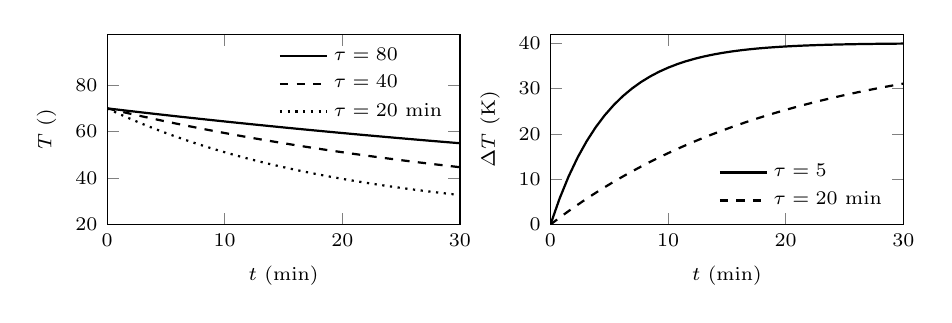
\begin{tikzpicture}
\begin{axis}[name=ret,width=0.50\linewidth,height=4.0cm,xmin=0,xmax=30,ymin=20,ymax=102,ytick={20,40,60,80},
 xlabel={$t$ (min)},ylabel={$T$ (\si{\celsius})},tick label style={font=\scriptsize},label style={font=\scriptsize},domain=0:30,samples=40,
 legend style={font=\scriptsize,draw=none,fill=none,at={(0.99,0.99)},anchor=north east},legend cell align=left]
\addplot[thick] {22+48*exp(-x/80)}; \addlegendentry{$\tau=80$}
\addplot[thick,dashed] {22+48*exp(-x/40)}; \addlegendentry{$\tau=40$}
\addplot[thick,dotted] {22+48*exp(-x/20)}; \addlegendentry{$\tau=20$ min}
\end{axis}
\begin{axis}[at={(ret.east)},anchor=west,xshift=1.15cm,width=0.50\linewidth,height=4.0cm,xmin=0,xmax=30,ymin=0,ymax=42,
 xlabel={$t$ (min)},ylabel={$\Delta T$ (K)},tick label style={font=\scriptsize},label style={font=\scriptsize},domain=0:30,samples=40,
 legend style={font=\scriptsize,draw=none,fill=none,at={(0.98,0.02)},anchor=south east},legend cell align=left]
\addplot[thick] {40*(1-exp(-x/5))}; \addlegendentry{$\tau=5$}
\addplot[thick,dashed] {40*(1-exp(-x/20))}; \addlegendentry{$\tau=20$ min}
\end{axis}
\end{tikzpicture}
\end{reffig}

\subsection{Measurement, fitting, validation}\label{sec:devicecal}
\CORE{} Universal good practice (not a rule):
\begin{enumerate}
\item \textbf{Preserve raw data}: time, temperature, ambient (start and end), water volume or mass, configuration, thermometer ID. Never overwrite readings with fitted values.
\item \textbf{Control} the measured quantity: same volume, probe position and depth, stirring before reading, lid state.
\item \textbf{Repeat} each condition ($\ge3$ trials) and vary initial temperature across the range you may face; record ambient drift.
\item \textbf{Fit} a suitable model: $\ln(T-T_{\text{amb}})$ vs $t$ (\eqp{F:transfer:semilog}), or an empirical calibration line of final temperature vs initial temperature at the specified duration (fewer assumptions, valid only inside the tested range).
\item \textbf{Check residuals} for curvature and outliers; check repeatability (standard deviation of repeats); correct for ambient by working with $T-T_{\text{amb}}$.
\item \textbf{Validate} on trials withheld from the fit; report prediction error.
\item \textbf{Report extrapolation separately}; note sensor lag (\pg{sec:constinput}).
\end{enumerate}

\textbf{Two different uncertainties.} For a straight-line fit with $n$ points, residual standard deviation $s$, the uncertainty of the \emph{mean} response at $x_0$ scales as $s\sqrt{1/n+(x_0-\bar x)^2/S_{xx}}$, while a \emph{single new trial} scatters by $s\sqrt{1+1/n+(x_0-\bar x)^2/S_{xx}}$ (a prediction interval, always wider; $S_{xx}=\sum(x_i-\bar x)^2$).\src{EK} Predicting tomorrow's one run needs the second.

\begin{trapbox}\anchor{trap:safety}\textbf{Safety.} Hot water scalds; use tongs/mitts and stable bases. Never seal a container that will be heated (pressure build-up). No improvised electrical heaters or modified mains devices. Avoid thermal shock to glass (sudden large $\Delta T$). Follow every energy-source and material restriction in the official rules.\end{trapbox}
\end{multicols}

\begin{reftab}{T:devicelog}{Calibration record (blank template; one row per trial).}
\small
\renewcommand{\arraystretch}{1.55}
\begin{tabularx}{\textwidth}{@{}|C{0.05\textwidth}|C{0.09\textwidth}|Y|C{0.08\textwidth}|C{0.11\textwidth}|C{0.07\textwidth}|C{0.07\textwidth}|C{0.07\textwidth}|C{0.13\textwidth}|@{}}
\hline
Trial & Date/time & Setup / changes & Volume (mL) & $T_{\text{amb}}$ start/end (\si{\celsius}) & $T_0$ (\si{\celsius}) & $t$ (min) & $T_{\text{end}}$ (\si{\celsius}) & Prediction / notes\\
\hline
 & & & & & & & & \\ \hline
 & & & & & & & & \\ \hline
 & & & & & & & & \\ \hline
 & & & & & & & & \\ \hline
 & & & & & & & & \\ \hline
 & & & & & & & & \\ \hline
\end{tabularx}\end{reftab}
